\section{ASCbase::hbond\_\-ideal\_\-point\_\-t Class Reference}
\label{classASCbase_1_1hbond__ideal__point__t}\index{ASCbase::hbond_ideal_point_t@{ASCbase::hbond\_\-ideal\_\-point\_\-t}}
An \char`\"{}ideal\char`\"{} hbond point.  


{\tt \#include $<$hbond\_\-points.H$>$}

Inheritance diagram for ASCbase::hbond\_\-ideal\_\-point\_\-t::\begin{figure}[H]
\begin{center}
\leavevmode
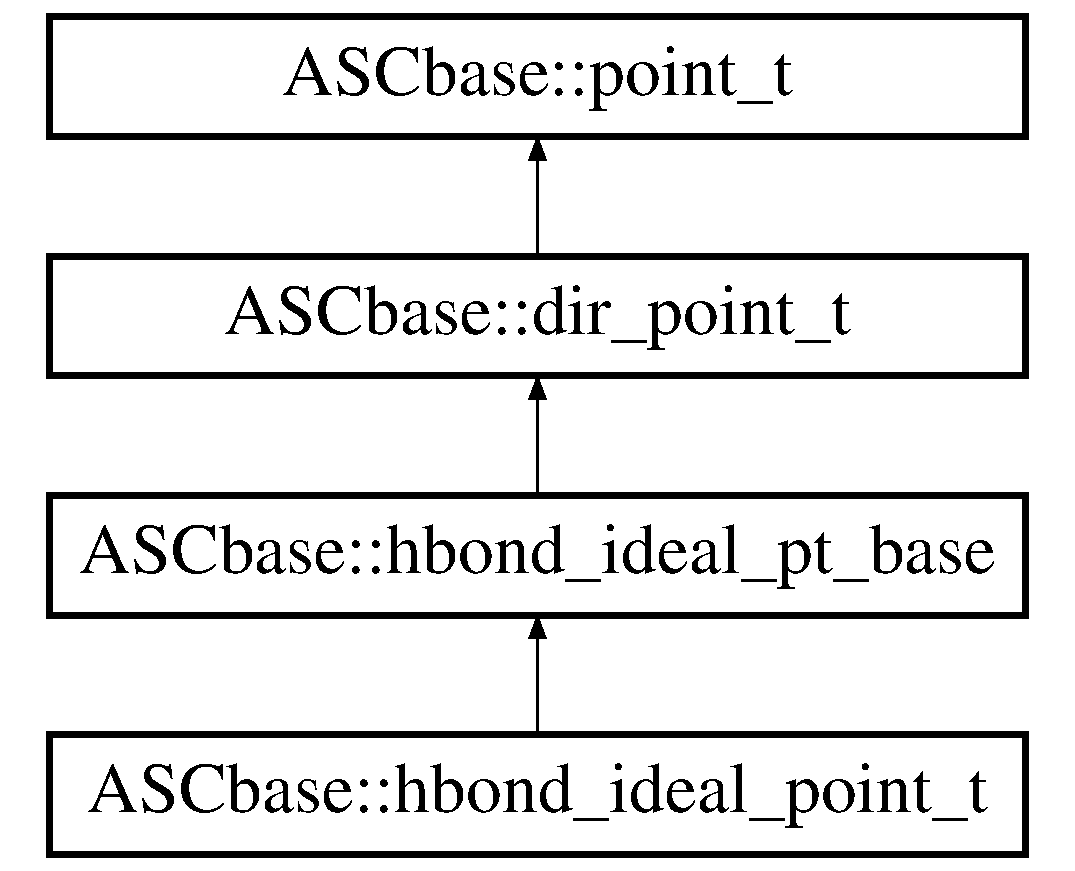
\includegraphics[height=4cm]{classASCbase_1_1hbond__ideal__point__t}
\end{center}
\end{figure}
\subsection*{Public Member Functions}
\begin{CompactItemize}
\item 
\textbf{hbond\_\-ideal\_\-point\_\-t} (alloc\_\-t a=ALLOC\_\-POSITION)\label{classASCbase_1_1hbond__ideal__point__t_17edfda196584b6b9f2bd4c26ada8d7a}

\item 
\textbf{hbond\_\-ideal\_\-point\_\-t} (const \bf{hbond\_\-ideal\_\-point\_\-t} \&p)\label{classASCbase_1_1hbond__ideal__point__t_51934c9d9788021b09d2d24eb5b976e7}

\item 
const \bf{hbond\_\-ideal\_\-point\_\-t} \& \textbf{operator=} (const \bf{hbond\_\-ideal\_\-point\_\-t} \&p)\label{classASCbase_1_1hbond__ideal__point__t_9fcb68e2f672eebb7505ed413123a78c}

\end{CompactItemize}
\subsection*{Public Attributes}
\begin{CompactItemize}
\item 
hbond\_\-fit\_\-pt\_\-vci \bf{fit\_\-pts\_\-beg}\label{classASCbase_1_1hbond__ideal__point__t_620a62e5bfaeb61bc5815745a60aed5c}

\begin{CompactList}\small\item\em Const iter to the first fit point corresponding to this ideal point. \item\end{CompactList}\item 
hbond\_\-fit\_\-pt\_\-vci \bf{fit\_\-pts\_\-end}\label{classASCbase_1_1hbond__ideal__point__t_fd82444a9d7addc28b06b24e9b9badee}

\begin{CompactList}\small\item\em Const iter to 1 past the end of the fit points corresponding to this ideal point. \item\end{CompactList}\end{CompactItemize}
\subsection*{Private Member Functions}
\begin{CompactItemize}
\item 
void \textbf{do\_\-copy} (const \bf{hbond\_\-ideal\_\-point\_\-t} \&p)\label{classASCbase_1_1hbond__ideal__point__t_7cc7e353e9bce5777ffdf83cda34778b}

\end{CompactItemize}


\subsection{Detailed Description}
An \char`\"{}ideal\char`\"{} hbond point. 



The documentation for this class was generated from the following file:\begin{CompactItemize}
\item 
hbond\_\-points.H\end{CompactItemize}
